\documentclass{report}
\usepackage[utf8]{inputenc}
\usepackage{graphicx}
\usepackage{float}

\title{Content-Based Image Retrieval}
\author{Léo Vetter}

\begin{document}
  \maketitle

  \tableofcontents

  \chapter{Performance Evaluation}

  \section{Evaluation on Caldech datasets}

    \begin{figure}[H]
      \caption{Image Retrieval Performance on Caldech256}
      \centering
      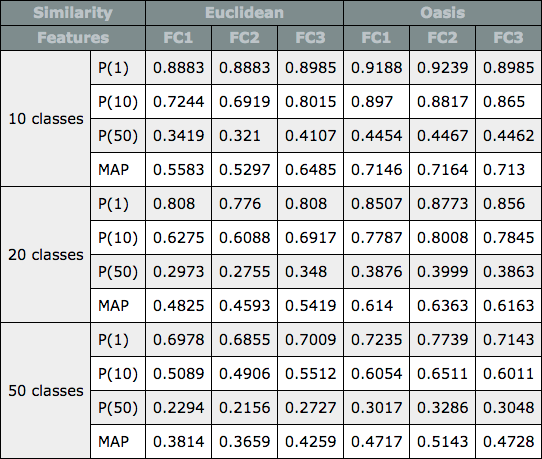
\includegraphics[scale=0.5]{images/evaluation/caldec_metrics_tables.png}
    \end{figure}

    \begin{figure}[H]
      \caption{Precision Curves on Caldech256}
      \centering
      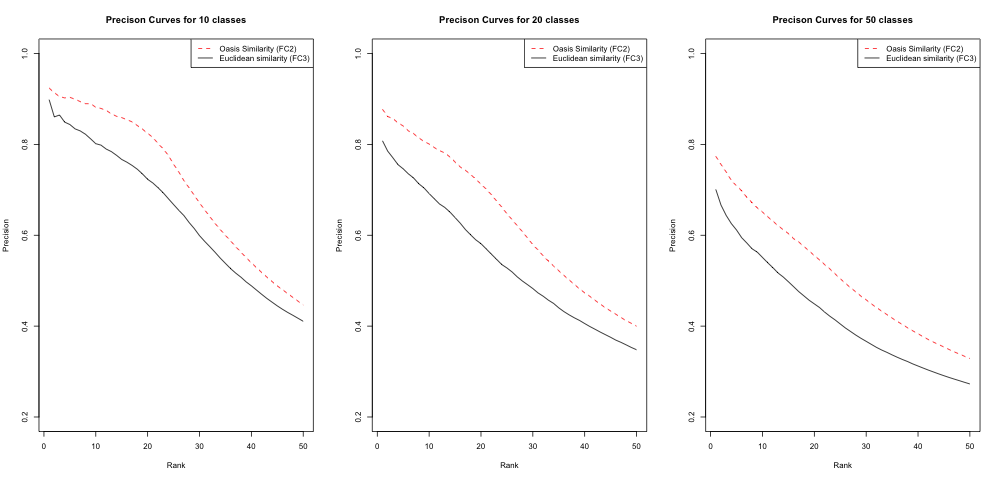
\includegraphics[scale=0.45]{images/evaluation/caldec_prec_curves.png}
    \end{figure}

  \section{Evaluation on Oxford datasets}

    \begin{figure}[H]
      \caption{Image Retrieval Performance on Oxford}
      \centering
      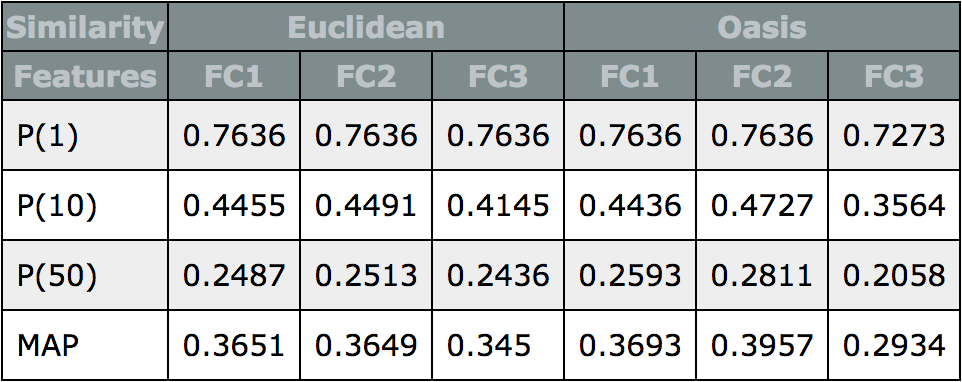
\includegraphics[scale=0.3]{images/evaluation/oxford_metrics_tables.png}
    \end{figure}

    \begin{figure}[H]
      \caption{Precision Curves on Oxford}
      \centering
      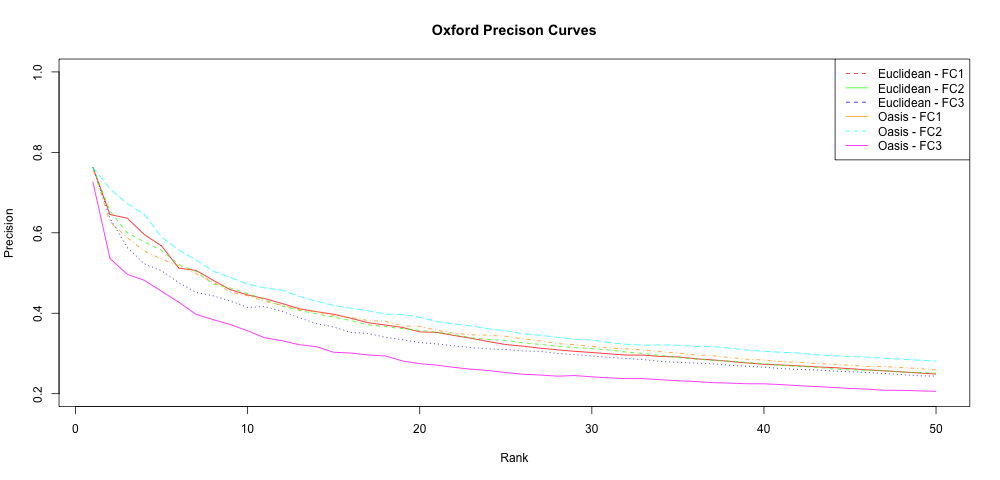
\includegraphics[scale=0.45]{images/evaluation/oxford_prec_curves.png}
    \end{figure}

    \section{Evaluation on Paris datasets}

      \begin{figure}[H]
        \caption{Image Retrieval Performance on Paris}
        \centering
        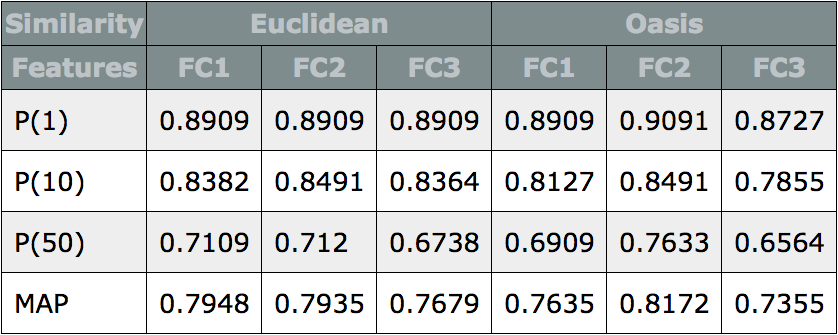
\includegraphics[scale=0.3]{images/evaluation/paris_metrics_tables.png}
      \end{figure}

      \begin{figure}[H]
        \caption{Precision Curves on Paris}
        \centering
        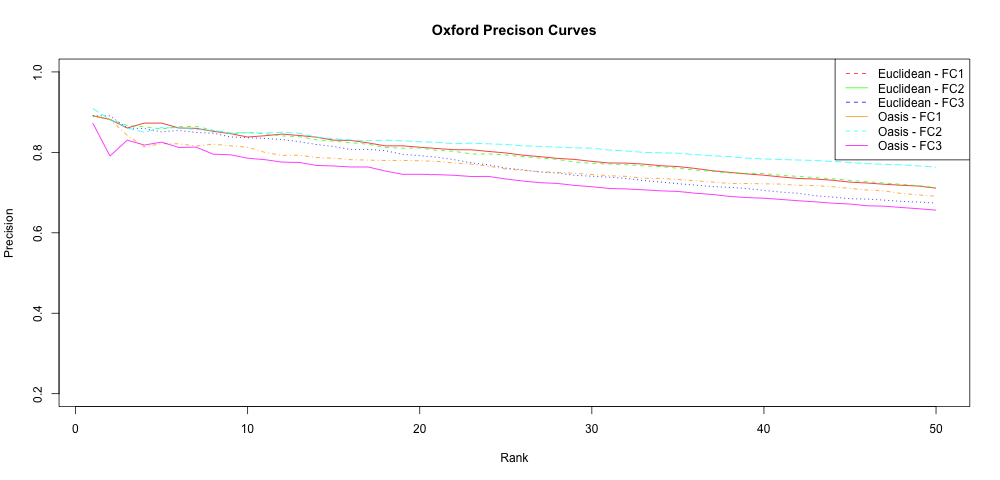
\includegraphics[scale=0.45]{images/evaluation/paris_prec_curves.png}
      \end{figure}

\end{document}
